\section{The IceCube Detector}
\label{sec:Detector}

The experimental data was taken at the IceCube experiment, located at the geographic South Pole at a depth of $\qtyrange{1450}{2450}{\metre}$.
The detector of IceCube consists of the in-ice array, DeepCore and IceTop and is used to detect high-energy neutrinos and muons.
It is formed by
86 cables each connected to 60 Digital Optical Modules (DOMs), consisting of a photomultiplier and a single-board computer, resulting in a total 
of 5160 photomultipliers detecting weak Cherenkov light of high-energy charged particles.\\
Seven of those cables are more densely packed with DOMs and form the DeepCore, which is needed to detect particles with lower energies with sufficient efficiency. While 
the energy threshold at the rest of the detector is approximately $\qty{100}{\giga\electronvolt}$, the DeepCore has an energy threshold of just $\approx \qty{10}{\giga\electronvolt}$.
This is achieved by the smaller distance and higher efficiency of the used photomultipliers.\\
The IceTop detector is used to detect air showers, which is both needed to study cosmic rays but also used as a veto, for detected particles in the in-ice array.
\begin{figure}
    \centering
    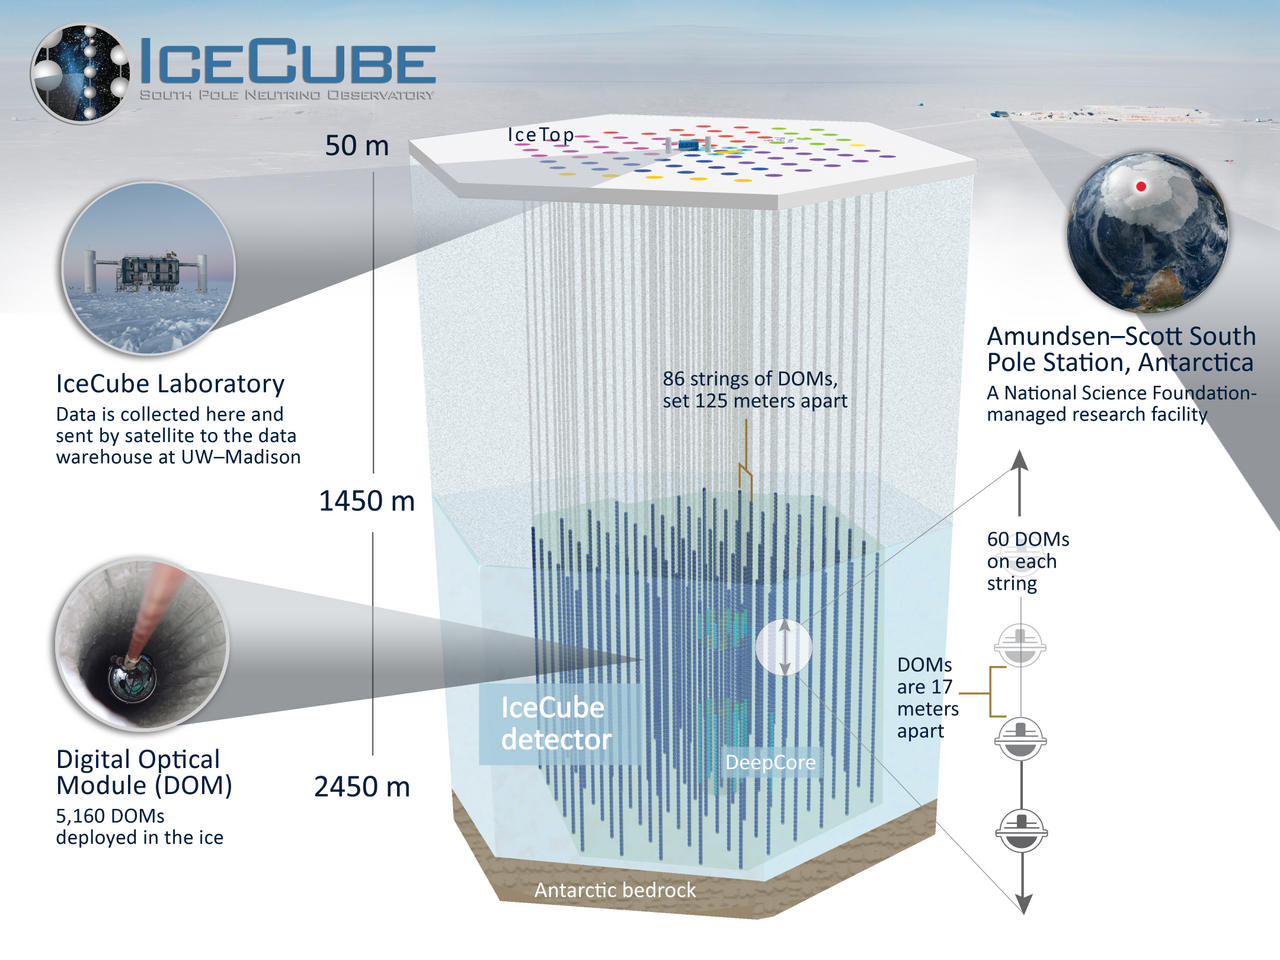
\includegraphics[width=0.7\textwidth]{content/pics/icecube_detector.jpg}
    \caption{A schematic view of the IceCube detector \cite{IceCube_pic}.}
    \label{fig:bb_oscillation}
\end{figure}

\section{Analysis Strategy}
\label{sec:Strategy}
In this analysis, \textit{starting events} are used to discard atmospheric muon events, since only cosmic neutrinos are of relevance. These \textit{starting events} come from neutrino
interactions within the detector and can therefore be used to distinguish between muons coming from the atmosphere and muons coming from interactions with neutrinos. Another strategy is 
to apply a cut on the reconstructed zenith angle, since atmospheric muons cannot come from below the detector (traveling through earth).
Since the reconstruction of the direction of the event is not precise enough, the cut only improves the signal-to-noise ratio up to $1:10^3$. For further separation, machine learning
methods are used to distinguish between events deriving from astrophysical neutrinos (signal) and those, that have been incorrectly reconstructed.\\
To train a classifier for signal-background separation, the data has to be properly prepared first. For this, any attributes consisting of mostly \texttt{NaN}s or \texttt{Inf}s are discarded.
A Monte Carlo simulation of signal and background events is used to train the classifier. Therefore, any attributes only appearing in either the simulation or the real recorded data are
discarded as well. Also, unphysical parameters (e.g Monthe Carlo truth attributes with names \texttt{Weight, MC, Corsika, I3EventHeader}) are not suited for the training process. The \texttt{label}
attribute of the simulation includes binary values for either signal (\texttt{1}) or background (\texttt{0}).\\
The given dataset includes $\approx 100$ attributes. An attribute selection is performed, to reduce the dimensionality and computing time for the classification task. For this, the mRMR method explained
in \ref{subsec:mRMR} is applied. After extracting the most useful features, a multivariate learner is trained to efficiently separate signal and background. In this analysis, a \textit{na\"ive Bayes classifier},
a \textit{Random Forest classifier}, as well as a \textit{kNN classifier} are trained and evaluated using the Precision and Recall for different thresholds $\tau_c$. The best threshold is then chosen by 
using the $f_{\beta}$ score. Additionally, ROC curves are plotted and the area under the ROC curve $A_{\mathrm{ROC}}$ is calculated to evaluate the classifier performance independently of the threshold.\\
The final labels of the real data are then predicted by the model with the best achieved performance.
